% !TeX root = main.tex
\documentclass[
    11pt,
    usenames, dvipsnames,
    usepdftitle=false,
    aspectratio=169,
]{beamer}
\graphicspath{{graphics/}{./}}
\newcommand{\Title}{Anticipatory Power Flow}
\newcommand{\Subtitle}{Formulation, Computation, and Applications}
\newcommand{\CYC}{Christian Y. Cahig}
\newcommand{\WorkEmail}{christian.cahig@outlook.com}
\newcommand{\ToWorkEmail}{mailto:christian.cahig@outlook.com}
\newcommand{\GitHub}{christian-cahig}
\newcommand{\ToGitHub}{https://github.com/christian-cahig}
\newcommand{\University}{Mindanao State University~--~Iligan Institute of Technology}
\newcommand{\Department}{Department of Electrical Engineering}

% Presentation information
\title[\Title]{\Title}
\subtitle{\Subtitle}
\author[C. Y. Cahig]{\CYC}
\institute[MSU~--~IIT]{
    % \Department \\
    \University \\ \smallskip
    {\faEnvelope \ \href{\ToWorkEmail}{\WorkEmail}}
    \quad
    {\faGithub \ \href{\ToGitHub}{christian-cahig}}
}
\date[23 November 2022]{}

% Colours
\definecolor{CitationColour}{HTML}{9F1D35}
\definecolor{InternalLinkColour}{HTML}{01796F}
\definecolor{URLColour}{HTML}{0D98BA}
\definecolor{CornellRed}{rgb}{0.7, 0.11, 0.11}
\definecolor{BrandeisBlue}{rgb}{0.0, 0.44, 1.0}
\definecolor{LightSalmon}{rgb}{1.0, 0.63, 0.48}
\definecolor{AtomicTangerine}{rgb}{1.0, 0.6, 0.4}

% Beamer customs
\usetheme{Boadilla}
\usefonttheme{professionalfonts}
\useinnertheme{rounded}
\setbeamertemplate{navigation symbols}{}
\setbeamertemplate{bibliography item}{\insertbiblabel}
\setbeamertemplate{enumerate items}[square]
% \setbeamercovered{transparent}
\usecolortheme{seahorse}
\makeatletter
\setbeamertemplate{footline}{
  \leavevmode%
  \hbox{%
    \begin{beamercolorbox}[wd=.333333\paperwidth,ht=2.25ex,dp=1ex,center]{author in head/foot}%
      \usebeamerfont{author in head/foot}\insertshortauthor~(\insertshortinstitute)
    \end{beamercolorbox}%
    \begin{beamercolorbox}[wd=.333333\paperwidth,ht=2.25ex,dp=1ex,center]{title in head/foot}%
      \usebeamerfont{title in head/foot}\let\hyperlink\@secondoftwo\insertshorttitle
    \end{beamercolorbox}%
    \begin{beamercolorbox}[wd=.333333\paperwidth,ht=2.25ex,dp=1ex,center]{date in head/foot}%
      \usebeamerfont{date in head/foot}\let\hyperlink\@secondoftwo\insertshortdate
    \end{beamercolorbox}%
  }%
  \vskip0pt%
}
\makeatother
\expandafter\def\expandafter\insertshortdate\expandafter{%
  \insertshortdate\hfill%
  \insertframenumber\,/\,\inserttotalframenumber}

% Maths
\usepackage{amsmath,amssymb,amsfonts}
\usepackage{mathtools,mismath,derivative,stmaryrd,steinmetz}
\usepackage{interval}
\usepackage{ieeetrantools}
\usepackage{xfrac}

% Fonts
\usepackage[utf8]{inputenc}

% Tables
\usepackage{booktabs,tabularx}

% Figures
\usepackage{caption}

% Hyperlinks
\hypersetup{
    pdftitle={\Title: \Subtitle},
    pdftitle={\CYC},
    colorlinks=true,
    hyperfootnotes=true,
    citecolor=CitationColour,
    linkcolor=InternalLinkColour,
    unicode,
}

% References
\usepackage[%
    sorting=none,
    citestyle=numeric-comp,
    firstinits=true,
    maxbibnames=3,
    maxcitenames=3,
    backref=true,
]{biblatex}
\addbibresource{references.bib}

% Texts
\usepackage{xspace,pifont,fontawesome5}

% Miscellaneous packages
\usepackage{ifthen}

% Spacing
% \setlength\abovecaptionskip{-1pt}
% \setlength\belowcaptionskip{-1pt}

% Phrases and texts
\newcommand{\eg}{\textit{e.g.}\xspace}
\newcommand{\ie}{\textit{i.e.}\xspace}
\newcommand{\etc}{\textit{etc.}\xspace}
\newcommand{\wrt}[1][]{\ifthenelse{\equal{#1}{full}}{with respect to\xspace}{wrt\xspace}}
\newcommand{\TextPlus}{\raisebox{\dimexpr(\fontcharht\font`X-\height+\depth)/2\relax}{+}}
\newcommand{\XED}[1][]{%
\ifthenelse{\equal{#1}{full}}{%
  extended economic dispatch\xspace}{%
  ED\TextPlus\xspace}%
}
\newcommand{\APFE}[1][]{%
\ifthenelse{\equal{#1}{full}}{%
  APF equations\xspace}{%
  PFE\TextPlus\xspace}%
}
\newcommand{\ctpb}{\textit{ceteris paribus}\xspace}

% Tables
\newcolumntype{L}{>{\raggedright\arraybackslash}X}
\newcolumntype{C}{>{\centering\arraybackslash}X}
\newcolumntype{R}{>{\raggedleft\arraybackslash}X}
\setlength\heavyrulewidth{0.25ex}

% Constants
\newcommand{\ImagUnit}{\mathup{j}}
\newcommand{\EulerConst}{\mathup{e}}

% Operators
\DeclarePairedDelimiter{\AbsVal}{\lvert}{\rvert}
\newcommand{\Diag}[1]{\operatorname{Diag}\paren{#1}}
\newcommand{\Conj}[1]{\operatorname{conj}\paren{#1}}
\DeclarePairedDelimiter{\Norm}{\lVert}{\rVert}
\newcommand{\RePart}[1]{\operatorname{Re}\paren{#1}}
\newcommand{\ImPart}[1]{\operatorname{Im}\paren{#1}}
\newcommand{\Sum}[1]{\operatorname{sum}\paren{#1}}
\newcommand{\Clip}[3]{\operatorname{clip}\paren{#2,#1,#3}}

% Vectors and matrices
\newcommand{\RealMat}[1]{\boldsymbol{\MakeUppercase{#1}}}
\newcommand{\RealVec}[1]{\boldsymbol{\MakeLowercase{#1}}}
\newcommand{\Zeros}{\boldsymbol{0}}
\newcommand{\Ones}{\boldsymbol{1}}
\newcommand{\ZerosVec}[1][]{\ifthenelse{\equal{#1}{}}{\Zeros}{\Zeros_{#1}}}
\newcommand{\ZerosMat}[2]{\ifthenelse{\equal{#1}{}}{\Zeros}{\Zeros_{#1,#2}}}
\newcommand{\OnesVec}[1][]{\ifthenelse{\equal{#1}{}}{\Ones}{\Ones_{#1}}}
\newcommand{\OnesMat}[2]{\ifthenelse{\equal{#1}{}}{\Ones}{\Ones_{#1,#2}}}

% Sets
\newcommand{\Reals}{\mathbb{R}}
\newcommand{\Cplxs}{\mathbb{C}}
\newcommand{\Buses}{\mathcal{N}}
\newcommand{\Branches}{\mathcal{E}}
\newcommand{\GridGraph}{\left(\Buses,\Branches\right)}
\newcommand{\SupUnits}{\mathcal{U}}
\newcommand{\SData}{\mathcal{S}}
\newcommand{\DData}{\mathcal{D}}
\newcommand{\IData}{\mathcal{I}}
\newcommand{\PData}{\mathcal{P}}

% Counts
\newcommand{\NumBuses}{N}
\newcommand{\NumBranches}{E}
\newcommand{\NumSupUnits}{U}
\newcommand{\NumDemUnits}{D}

% Admittance matrix
\newcommand{\Ybus}{\boldsymbol{Y}}
\newcommand{\Gbus}{\boldsymbol{G}}
\newcommand{\Bbus}{\boldsymbol{B}}
\newcommand{\GBbus}{\Gbus + \ImagUnit\Bbus}

% Supply units
\newcommand{\SupPs}{\boldsymbol{p}_{\mathsf{u}}}
\newcommand{\SupQs}{\boldsymbol{q}_{\mathsf{u}}}
\newcommand{\SupSs}{\SupPs + \ImagUnit\SupQs}
\newcommand{\SupInjs}{\boldsymbol{c}}
\newcommand{\SupPQs}{\left(\SupPs,\SupQs\right)}
\newcommand{\SupCon}{\boldsymbol{C}_{\!\mathsf{u}}}
\newcommand{\SupP}[1]{p_{\mathsf{u,}#1}}
\newcommand{\SupQ}[1]{p_{\mathsf{u,}#1}}
\newcommand{\SnapSupPs}{\widetilde{\boldsymbol{p}}_{\mathsf{u}}}
\newcommand{\SnapSupQs}{\widetilde{\boldsymbol{q}}_{\mathsf{u}}}
\newcommand{\SnapSupInjs}{\widetilde{\boldsymbol{c}}}
\newcommand{\SupPmins}{\underline{\boldsymbol{p}_{\mathsf{u}}}}
\newcommand{\SupQmins}{\underline{\boldsymbol{q}_{\mathsf{u}}}}
\newcommand{\SupPQmins}{\left(\SupPmins,\SupQmins\right)}
\newcommand{\SupPmaxs}{\overline{\boldsymbol{p}_{\mathsf{u}}}}
\newcommand{\SupQmaxs}{\overline{\boldsymbol{q}_{\mathsf{u}}}}
\newcommand{\SupPQmaxs}{\left(\SupPmaxs,\SupQmaxs\right)}
\newcommand{\SupInjmins}{\underline{\SupInjs}}
\newcommand{\SupInjmaxs}{\overline{\SupInjs}}

% Demand units
\newcommand{\DemPs}{\boldsymbol{p}_{\mathsf{d}}}
\newcommand{\DemQs}{\boldsymbol{q}_{\mathsf{d}}}
\newcommand{\DemSs}{\DemPs + \ImagUnit\DemQs}
\newcommand{\DemDrws}{\boldsymbol{d}}
\newcommand{\DemPQs}{\left(\DemPs,\DemQs\right)}
\newcommand{\DemCon}{\boldsymbol{C}_{\!\mathsf{d}}}
\newcommand{\SnapDemPs}{\widetilde{\boldsymbol{p}}_{\mathsf{d}}}
\newcommand{\SnapDemQs}{\widetilde{\boldsymbol{q}}_{\mathsf{d}}}
\newcommand{\SnapDemDrws}{\widetilde{\boldsymbol{d}}}

% Bus voltages
\newcommand{\BusMs}{\boldsymbol{\upsilon}}
\newcommand{\BusAs}{\boldsymbol{\delta}}
\newcommand{\BusVs}[1][]{%
\ifthenelse{\equal{#1}{euler}}{%
  \BusMs\EulerConst^{\ImagUnit\BusAs}}{%
  \BusMs\phase{\BusAs}}%
}
\newcommand{\BusVolts}{\boldsymbol{s}}
\newcommand{\BusMAs}{\left(\BusMs,\BusAs\right)}
\newcommand{\BusM}[1]{\upsilon_{#1}}
\newcommand{\BusA}[1]{\delta_{#1}}
\newcommand{\SnapBusMs}{\widetilde{\boldsymbol{\upsilon}}}
\newcommand{\SnapBusAs}{\widetilde{\boldsymbol{\delta}}}
\newcommand{\SnapBusVolts}{\widetilde{\boldsymbol{s}}}
\newcommand{\BranchAs}{\boldsymbol{\varphi}}

% Net nodal injections
\newcommand{\NetPs}{\boldsymbol{p}}
\newcommand{\NetQs}{\boldsymbol{q}}
\newcommand{\NetPQs}{\NetPs + \ImagUnit\NetQs}
\newcommand{\NetInjs}{\boldsymbol{e}}

% Nodal residuals
\newcommand{\Resids}{\boldsymbol{\phi}}

% ED+
\newcommand{\XEDObj}[1]{%
\ifthenelse{\equal{#1}{loss}}{%
  f_{\mathsf{loss}}}{\ifthenelse{\equal{#1}{reg}}{%
  f_{\mathsf{reg}}}{%
  f_{\mathsf{loss}} + f_{\mathsf{reg}}}}%
}
\newcommand{\XEDReg}[1]{\ifthenelse{\equal{#1}{p}}{\mu_{\mathsf{p}}}{\mu_{\mathsf{q}}}}
\newcommand{\XEDRegs}{\left(\XEDReg{p},\XEDReg{q}\right)}
\newcommand{\XEDShun}[1]{\operatorname{shunt}\paren{#1}}
\newcommand{\XEDLoss}[1]{\operatorname{loss}\paren{#1}}

% PFE+
\newcommand{\PFEVars}{\boldsymbol{x}}
\newcommand{\PFERefBus}{\hat{n}}
\newcommand{\PFERefA}{\BusA{\mathsf{ref}}}
\newcommand{\PFEBusAs}{\boldsymbol{\vartheta}}
\newcommand{\PFESlack}{\kappa}
\newcommand{\PFESDist}{\boldsymbol{\PFESlack}}
\newcommand{\PFEResids}{\boldsymbol{\psi}}

% OPF
\newcommand{\OPFVars}[1][]{%
\ifthenelse{\equal{#1}{}}{%
  \left(\SupInjs,\BusVolts\right)}{
  \left(\SupInjs_{#1},\BusVolts_{#1}\right)}%
}
\newcommand{\OPFVar}[2]{%
\ifthenelse{\equal{#1}{c}}{%
  \SupInjs_{#2}}{%
  \BusVolts_{#2}}%
}
\newcommand{\Optim}[2][]{%
\ifthenelse{\equal{#1}{s}}{%
  #2^{\star}_{\mathsf{s}}}{%
  #2^{\star}_{\mathsf{w}}}%
}

% Derivatives
\newcommand{\Gradient}[2]{\nabla_{#2}#1}

% General APF
\newcommand{\APFJac}[1][]{\ifthenelse{\equal{#1}{b}}{\boldsymbol{H}}{\boldsymbol{J}}}
\newcommand{\APFPoint}{\left(\SupInjs,\PFEVars\right)}
\newcommand{\SnapPoint}{\left(\SnapSupInjs,\SnapBusVolts\right)}
\newcommand{\APFBGrad}{\boldsymbol{g}}




% Document proper
\begin{document}

\section{Front matter}
\begin{frame}[t]\titlepage\end{frame}   % Title slide

\section{Preliminaries}
\subsection{System model}

\begin{frame}[t]{The steady-state grid as a weighted graph \(\GridGraph\)}{}
    \onslide*<1-3>{
    \textcolor<1>{CornellRed}{\(\NumBuses\) buses} as nodes,
    \textcolor<1>{CornellRed}{\(\NumBranches\) branches} as edges,
    \begin{itemize}
        \item \(\Buses\): key locations (\eg, substation)
        \item \(\Branches\): bus-to-bus interfaces (\eg, lines, cables, transformers)
    \end{itemize}

    \vspace{1em}
    \textcolor<2>{CornellRed}{Branch admittances} act as edge weights
    \begin{itemize}
        \item How well a branch admits power flow
    \end{itemize}

    \vspace{1em}
    \textcolor<3>{CornellRed}{Bus admittance matrix \(\Ybus=\GBbus\)} act as graph Laplacian
    \begin{itemize}
        \item Sparsity reflects grid topology
        \item Elements computed from admittances
        \item[\ding{43}] \(\Ybus\) encodes \textcolor<3>{CornellRed}{grid intrinsics}
    \end{itemize}
    }

    \onslide*<4->{
    Buses are entry and exit points for power
    \begin{itemize}
        \item Demand units \textcolor<4>{CornellRed}{draw \(\DemSs \in \Cplxs^{\NumSupUnits}\)}
        \item Supply units \textcolor<4>{CornellRed}{inject \(\SupSs \in \Cplxs^{\NumDemUnits}\)}
        \item \(\SupCon\), \(\DemCon\): connection matrices
        \item \(\DemDrws \coloneqq \DemPQs\) and \(\SupInjs \coloneqq \SupPQs\)
        \item[\ding{43}] Net nodal injections:
            \textcolor<4>{CornellRed}{\(\SupCon\left(\SupSs\right) - \DemCon\left(\DemSs\right)\)}
    \end{itemize}

    \vspace{1em}
    Bus voltages \textcolor<5>{CornellRed}{\(\BusVs\equiv\BusVs[euler]\)}
    are \textcolor<5>{CornellRed}{state variables}
    \begin{itemize}
        \item For a grid with \(\Ybus\), its state is computable given
            \(\BusVolts \coloneqq \BusMAs\)
        \item[\ding{43}] Net nodal injections:
            \textcolor<5>{CornellRed}{\(\Diag{\BusVs} \, \Conj{\Ybus\BusVs}\)}
    \end{itemize}
    }
\end{frame}

\subsection{Power flow equations}

\begin{frame}[t]{Power flow equations (PFE)}{%
    The standard model of steady-state grid physics}
    \begin{block}{Nodal power balance}{}
        \vspace{-1em}
        \begin{IEEEeqnarray*}{rCl}
            \Diag{\BusVs} \, \Conj{\Ybus\BusVs}
            & = &
            \SupCon\left(\SupSs\right) - \DemCon\left(\DemSs\right)
        \end{IEEEeqnarray*}
        % 
        or, equivalently, as a system of \(2\NumBuses\) nonlinear equations,
        % 
        {\color{CornellRed}\begin{IEEEeqnarray*}{rCl}
            \begin{bmatrix*}[r]
                \Diag{\BusMs\odot\cos\BusAs} & \Diag{\BusMs\odot\sin\BusAs} \\
                \Diag{\BusMs\odot\sin\BusAs} & -\Diag{\BusMs\odot\cos\BusAs}
            \end{bmatrix*}
            \begin{bmatrix*}[r] \Gbus & -\Bbus\, \\ \Bbus & \Gbus\, \end{bmatrix*}
            \begin{bmatrix*} \BusMs\odot\cos\BusAs\, \\ \BusMs\odot\sin\BusAs\, \end{bmatrix*}
            & = &
            \begin{bmatrix*}
                \SupCon\SupPs - \DemCon\DemPs \\ \SupCon\SupQs - \DemCon\DemQs
            \end{bmatrix*}
        \end{IEEEeqnarray*}}
        \vspace{-1em}
    \end{block}

    \begin{itemize}
        \item Staple requirement in power flow analysis (PFA) computations

        \item PFE parameters:
            \(\Ybus\) as \textcolor<2>{CornellRed}{grid intrinsics},
            \(\DemDrws\) as \textcolor<2>{CornellRed}{external stimuli}

        \item \(\left(\SupInjs,\BusVolts\right)\) are
            \textcolor<3>{CornellRed}{power-flow feasible for \(\left(\Ybus,\DemDrws\right)\)}
            if they satisfy the PFE for \(\left(\Ybus,\DemDrws\right)\)
    \end{itemize}
\end{frame}

\subsection{Power flow manifold}

\begin{frame}[t]{Power flow manifold (PFM)}{%
    A geometric intuition for the PFE}

    \begin{block}{PFE as a manifold in \(\left(\SupInjs,\BusVolts\right)\)--space}
        Expressed as
        {\color{CornellRed}
        \(\Resids\paren{\SupInjs,\BusVolts;\Ybus,\DemDrws} \ = \ZerosVec[2\NumBuses]\)},
        the PFE describe a manifold of all points \(\left(\SupInjs,\BusVolts\right)\)
        that are power-flow feasible for \(\left(\Ybus,\DemDrws\right)\).
    \end{block}

    \begin{itemize}
        \item PFE parameters \(\left(\Ybus,\DemDrws\right)\)
            dictate the \textcolor<2>{CornellRed}{``shape'' of PFM}

        \item Power-flow feasible \(\left(\SupInjs,\BusVolts\right)\)
            for \(\left(\Ybus,\DemDrws\right)\)
            \(\Longrightarrow\)
            \textcolor<3>{CornellRed}{\(\left(\SupInjs,\BusVolts\right)\)
            is on PFM for \(\left(\Ybus,\DemDrws\right)\)}

        \item Computation over PFE for \(\left(\Ybus,\DemDrws\right)\)
            \(\Longrightarrow\)
            \textcolor<3>{CornellRed}{finding a point on PFM for \(\left(\Ybus,\DemDrws\right)\)}
    \end{itemize}

    \vspace{5em}
\end{frame}

\subsection{Finding points on the power flow manifold}

\begin{frame}[t]{Finding a point on the PFM}{}
    \begin{itemize}
        \item <1-> \textcolor<1>{CornellRed}{Standard power flow} (SPF)
            as completing a point on PFM
        \begin{itemize}
            \item \textcolor<1>{CornellRed}{Fix some coordinates} with slack-PV-PQ model (\S2.4.1)
            \begin{itemize}
                \item Find \(k\in\Buses\) with supply unit, set \(\BusA{k}\) as reference
                \item Assume \(\BusM{m}\) and \(\SupP{n}\) for
                    all \(m\in\Buses\) with supply units,
                    and all unit \(n\) at \(m \neq k\)
            \end{itemize}

            \item \textcolor<1>{CornellRed}{Complete the other coordinates} from PFE
        \end{itemize}

        \vspace{0.5em}
        \item <2-> \textcolor<2-3>{CornellRed}{Continuation power flow} (CPF)
            as finding points through PFMs
        \begin{itemize}
            \item \textcolor<2>{CornellRed}{Estimating stability limits}:
                \(\Resids\paren{\Ybus,\DemDrws_{i}} \, = \ZerosVec[2\NumBuses]\)
                with \(\DemDrws_{i} = \lambda_{i}\DemDrws_{\mathsf{base}}\)
                \cite{AjjarapuChristy1992,CanizaresAlvarado1993,Chiang+1995,GomezQuiles+2016,%
                Liu+2005,Avalos+2009}

            \item \textcolor<2>{CornellRed}{Branch-outage contingency}:
                \(\Resids\paren{\Ybus_{i},\DemDrws} \, = \ZerosVec[2\NumBuses]\)
                by
                \cite{FlueckDondeti2000,FlueckQiu2004,Matarucco+2004,MataruccoNetoAmancio2014}
        \end{itemize}

        \vspace{0.5em}
        \item <3-> \textcolor<3>{CornellRed}{Optimal power flow} (OPF)
            as finding the best point on PFM
        \begin{itemize}
            \item Best point minimizes \textcolor<3>{CornellRed}{operating cost \(g\!\OPFVars\)}
                subject to
            \begin{itemize}
                \item Supply capacity:
                    \(\underline{\SupInjs} \leq \SupInjs \leq \overline{\SupInjs}\)
                \item Allowable state:
                    \(\RealMat{A}\BusVolts \leq \RealVec{b}\)
            \end{itemize}

            \item \textcolor<3>{CornellRed}{Nonconvex} (due to PFE)
                and \textcolor<3>{CornellRed}{NP-hard}
                \cite{LavaeiLow2012,Lehmann+2016,BienstockVerma2019}
        \end{itemize}
    \end{itemize}
\end{frame}



\section{Overview of the study}
\subsection{Problem statement}

\begin{frame}[t]{PFA computation in the online setting}{}
    \begin{itemize}
        \item \textcolor<1>{CornellRed}{Snapshot data} of past operating point:
            \(\SnapPoint\) in response to \(\SnapDemDrws\)
        \begin{itemize}
            \item[\ding{43}] Direct or computed from measurements
        \end{itemize}

        \vspace{0.75em}
        \item Expected conditions for \textcolor<2-3>{CornellRed}{upcoming dispatch}
        \begin{itemize}
            \item \textcolor<2>{CornellRed}{Updated intrinsics \(\Ybus\)}
                from online parameter estimation \cite{Lateef2020,Vanin+2022v1}
            \item \textcolor<2>{CornellRed}{Anticipated demand \(\DemDrws\)} from forecast
            \item \textcolor<2>{CornellRed}{Supply limits \(\SupInjmins\), \(\SupInjmaxs\)}
                (\eg, schedule, ramp)
            \item[\ding{43}] \(\DemDrws \neq \SnapDemDrws\), \ie,
                \textcolor<3>{CornellRed}{\(\SnapPoint\) not on PFM for
                \(\left(\Ybus,\DemDrws\right)\)}
        \end{itemize}

        \vspace{0.75em}
        \item \textcolor<4>{CornellRed}{Invariant} roster of supply \& demand units
            (\ie, fixed \(\SupCon\) and \(\DemCon\))
    \end{itemize}

    \begin{alertblock}<5>{}
        Using the snapshot point \(\SnapPoint\), how do we find a point \(\APFPoint\)
        on the PFM for \(\left(\Ybus,\DemDrws\right)\)?
    \end{alertblock}
\end{frame}


\section{Formulation}
\subsection{Foundational notions}

\begin{frame}[t]{Pillars of anticipatory power flow (APF)}{}
    \begin{enumerate}
    \item <1->
    \(\SupInjs\) as \textcolor<1>{CornellRed}{control},
    \(\BusVolts\) as \textcolor<1>{CornellRed}{state},
    and
    \textcolor<1>{CornellRed}{\(\BusVolts\) as an implicit function of \(\SupInjs\)} via PFE
    \begin{itemize}
        \item OPF notion from '60s \cite[\S 2.4]{FrankRebennack2016};
            used in recent works on online OPF \cite{GanLow2016,Tang+2017}
        \item[\faLightbulb] Compute \(\SupInjs\) voltage-free,
            then solve for \(\BusVolts\) from PFE
    \end{itemize}

    \vspace{1em}
    \item <2->
    To \textcolor<2>{CornellRed}{avoid rotational degeneracy},
    pick \textcolor<2>{CornellRed}{any} bus \(\PFERefBus\) as reference
    and \(\BusA{\PFERefBus} \gets \PFERefA\)
    \begin{itemize}
        \item PFE are \textcolor<2>{CornellRed}{sinusoids of phase angle differences},
            not of phase angles
        \item Slack-PV-PQ is \textcolor<2>{CornellRed}{mathematically unnecessary}
            \cite[\S 2.2.1]{MolzahnHiskens2019}
        \item[\faLightbulb] Non-reference voltage phase angles:
            \(\PFEBusAs \in \Reals^{\NumBuses-1}\)
    \end{itemize}

    \vspace{1em}
    \item <3>
    To make \textcolor<3>{CornellRed}{solving PFE well-determined},
    add a \textcolor<3>{CornellRed}{distributed slack \(\PFESlack \in \Reals\)}
    \begin{itemize}
        \item Based on SPF notion \textcolor<3>{CornellRed}{distributed slack bus},
            dating back to '90s \cite{Meisel1993}
        \item \(\PFESlack\) shared via
            \textcolor<3>{CornellRed}{slack distribution ratios \(\PFESDist\)}
            based on supply limits (\S 3.3)
        \item[\faLightbulb] With
            \(\PFEVars\coloneqq\begin{bmatrix*}\BusMs;\PFEBusAs;\PFESlack\end{bmatrix*}\)
            as state variables, restate PFE as
            \(\Resids\paren{\PFEVars;\Ybus,\DemDrws,\SupInjs,\BusA{\PFERefBus}}
            \,=\ZerosVec[2\NumBuses]\)
    \end{itemize}
    \end{enumerate}
\end{frame}

\subsection{Solving for the anticipated supply injections}

\begin{frame}[t]{Solving for the anticipated supply injections}{}
    \begin{block}{Extended economic dispatch (\XED)}
    \vspace{-1em}
    \begin{align*}
        \operatornamewithlimits{min}_{\RealVec{p},\,\RealVec{q}}
        \quad &
        \underbrace{
            \Norm*{\begin{matrix*}\RealVec{p}\end{matrix*}}_{2}
            +
            \Norm*{\begin{matrix*}\RealVec{q}\end{matrix*}}_{2}
        }_{\XEDObj{loss}}
        \ + \
        \underbrace{
            \XEDReg{p} \Norm*{\begin{matrix*}\RealVec{p} - \SnapSupPs\end{matrix*}}_{2}
            +
            \XEDReg{q} \Norm*{\begin{matrix*}\RealVec{q} - \SnapSupQs\end{matrix*}}_{2}
            }_{\XEDObj{reg}} \\
        \operatorname{s.t.} \quad &
        \OnesVec^{\!\mathsf{T}} \RealVec{p} \,= p_{\mathsf{need}}, \quad
        \OnesVec^{\!\mathsf{T}} \RealVec{q} \,= q_{\mathsf{need}}, \quad
        \SupPmins \leq \RealVec{p} \leq \SupPmaxs, \quad
        \SupQmins \leq \RealVec{q} \leq \SupQmaxs,
        \\
        \operatorname{with} \quad &
        p_{\mathsf{need}} = \Clip{%
            \OnesVec^{\!\mathsf{T}} \DemPs + p_{\mathsf{h}} + p_{\mathsf{o}}%
        }{\OnesVec^{\!\mathsf{T}} \SupPmins}{\OnesVec^{\!\mathsf{T}} \SupPmaxs},
        \quad
        q_{\mathsf{need}} = \Clip{%
            \OnesVec^{\!\mathsf{T}} \DemQs + q_{\mathsf{h}} + q_{\mathsf{o}}%
        }{\OnesVec^{\!\mathsf{T}} \SupQmins}{\OnesVec^{\!\mathsf{T}} \SupQmaxs},
        \\
        \quad &
        p_{\mathsf{h}} + \ImagUnit q_{\mathsf{h}} = \XEDShun{\SnapBusMs,\SnapBusAs;\Ybus},
        \quad \operatorname{and} \quad
        p_{\mathsf{o}} + \ImagUnit q_{\mathsf{o}} = \XEDLoss{\SnapBusMs,\SnapBusAs;\Ybus}.
    \end{align*}
    \end{block}

    \begin{itemize}
        \item <1-> Vanilla ED but considers reactive powers
        \begin{itemize}
            \item <1-> \textcolor<1>{CornellRed}{Supply regularization
                \(\XEDReg{p},\XEDReg{q} \geq 0\)}
            \item <1-> \textcolor<2>{CornellRed}{Adjust for non-demand consumption}:
                \(\XEDShun{\cdot}\) (\S 3.2.1) and \(\XEDLoss{\cdot}\) (\S 3.2.2)
        \end{itemize}

        \item <3> \textcolor<3>{CornellRed}{Convex}:
            checked with CVX 2.2 \cite{CVX_v2.2}, has a convex QP form (\S 3.2.3)
        \begin{itemize}
            \item[\ding{43}] <3> Lots of well-established polynomial-time algorithms
        \end{itemize}
    \end{itemize}
\end{frame}

\subsection{Solving for the anticipated bus voltages}

\begin{frame}[t]{Solving for the anticipated bus voltages}{}
    \begin{block}{APF equations (\APFE)}
    \vspace{-1em}
    \begin{IEEEeqnarray*}{rCcCl}
        \Resids\paren{\PFEVars;\Ybus,\DemDrws,\SupInjs,\BusA{\PFERefBus}}
        &\coloneqq&
        \underbrace{
            \NetInjs \paren{\BusMs,\PFEBusAs;\Ybus,\BusA{\PFERefBus}}
            \ - \
            \PFESlack \begin{bmatrix*}\SupCon\PFESDist \\ \ZerosVec[\NumBuses]\end{bmatrix*}
        }_{\PFEResids\paren{\PFEVars;\,\Ybus,\,\BusA{\PFERefBus}}}
        -
        \begin{bmatrix*}\SupCon\SupPs \\ \SupCon\SupQs\end{bmatrix*}
        -
        \begin{bmatrix*}\DemCon\DemPs \\ \DemCon\DemQs\end{bmatrix*}
        &=&
        \ZerosVec[2\NumBuses]
    \end{IEEEeqnarray*}
    \end{block}

    \begin{itemize}
        \item <1-> A \textcolor<1>{CornellRed}{\(2\NumBuses\)--dimensional root-finding} task
        \begin{itemize}
            \item[\ding{43}] <1-> Lots of derivative-based algorithms with fast convergence guarantees
            \item <1-> See \S 3.3.2 for the \textcolor<1>{CornellRed}{APF Jacobian
                \(\APFJac\paren{\PFEVars} \,\coloneqq
                \partial_{\PFEVars}\PFEResids\paren{\PFEVars}\)}
            % \item <1-> See \S 3.3.3 for an initialization strategy
        \end{itemize}

        \item <2> \textcolor<2>{CornellRed}{\(\SupInjs\) is a parameter of \APFE}
        \begin{itemize}
            \item[\ding{43}] <2> Different \(\SupInjs\)'s give different \(\PFEVars\)'s
            \item[\ding{43}] <2> Compare APF points by their \(\PFESlack\)'s
        \end{itemize}
    \end{itemize}
\end{frame}


\section{Computation}
\subsection{Solvers and algorithms}

\begin{frame}[t]{Some fast solvers and algorithms for APF}{}
    \begin{columns}[T]
    \begin{column}{0.4\textwidth}
    For solving \XED
    \begin{itemize}
        \item \textcolor<1>{CornellRed}{SeDuMi} 1.3.4
            \cite{SeDuMi_v1.3.4,YeToddMizuno1994,Sturm1999}
        \item \textcolor<1>{CornellRed}{SDPT3} 4.0
            \cite{SDPT3_v4.0,Toh+1999,Tutuncu+2003}
        \item[\ding{43}] Free and open-source
        \item[\ding{43}] Shipped as part of CVX 2.2
    \end{itemize}
    \end{column}

    \pause
    \begin{column}{0.6\textwidth}
    For solving \APFE
    \begin{itemize}
        \item \textcolor<2>{CornellRed}{Powell hybrid method}
            \cite{Powell1968,Powell1970a,Powell1970b}
            % as used in MINPACK-1 \cite[\S 1.1, \S 2.2]{More+1980}
        \item \textcolor<2>{CornellRed}{Levenberg-Marquardt algorithm}
            \cite{Levenberg1944,Marquardt1963}
            % as described by \citeauthor{More1978} \cite{More1978}
        \item[\ding{43}] Quadratic local convergence
            \cite[\S 10.3, 11.2]{NocedalWright2006}
        \item[\ding{43}] Ready-to-use in modern solvers
    \end{itemize}
    \end{column}
    \end{columns}

    \pause
    \vspace{2em}
    \begin{center}
        \textcolor<3>{CornellRed}{APFLib}:
        a MATLAB library built on CVX and as an extension for MATPOWER

        {\href{https://github.com/christian-cahig/Masterarbeit-DemoApps}{%
        \faGithub \ christian-cahig/Masterarbeit-DemoApps}}
    \end{center}
\end{frame}

\subsection{Run time evaluations}

\begin{frame}[t]{Run time evaluations for solving \XED}{%
    Based on Intel Core i7-10750H CPU @ 2.60GHz w/ 16GB RAM}
    \texttt{ACT500}, \texttt{RTE1888}, and \texttt{POL3375}
    have 90, 298, and 596 supply units, respectively.
    \begin{figure} 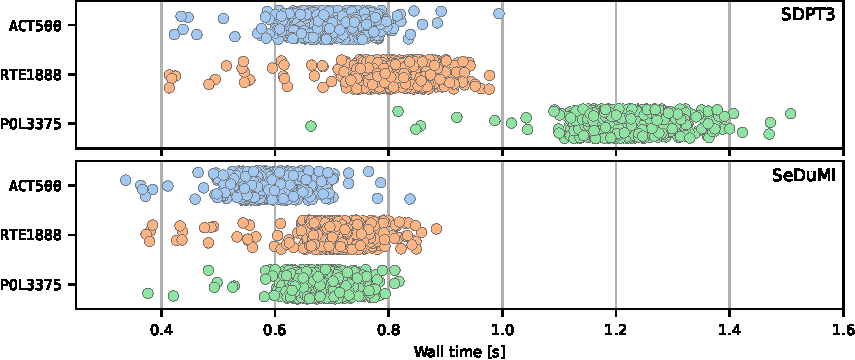
\includegraphics[width=0.95\textwidth]{apf1-times.pdf} \end{figure}
\end{frame}

\begin{frame}[t]{Run time evaluations for solving \APFE}{%
    Based on Intel Core i7-10750H CPU @ 2.60GHz w/ 16GB RAM}
    \texttt{ACT500}, \texttt{RTE1888}, and \texttt{POL3375}
    have 500, 1888, and 3374 buses, respectively.
    \begin{figure} 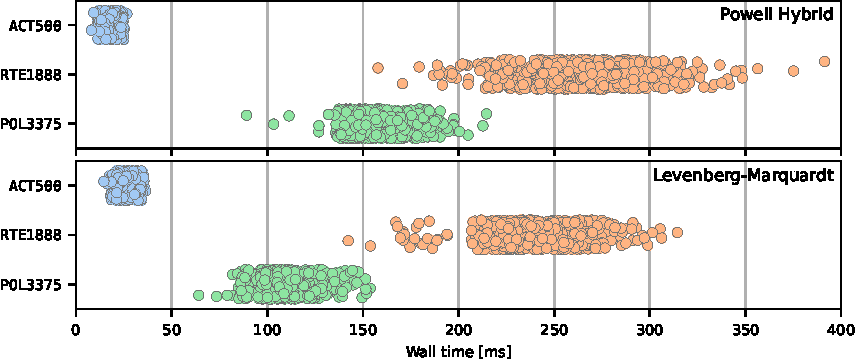
\includegraphics[width=0.95\textwidth]{apf2-times.pdf} \end{figure}
\end{frame}

\subsection{Effect of the supply regularization strengths}

\begin{frame}[t]{Effect of supply regularization on the APF point}{}
    \onslide*<1-4>{
    All else fixed, what happens to \(\APFPoint\) when
    \(\XEDRegs \in \left\{0,10^{-4},1\right\} \times \left\{0,10^{-4},1\right\}\)?
    }
    \onslide*<2>{
    \begin{figure} 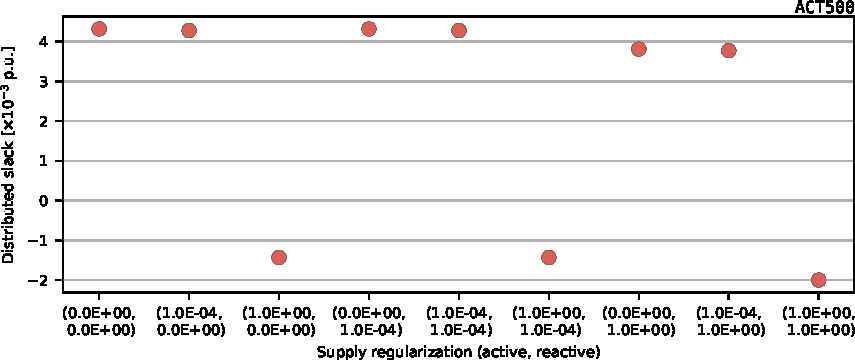
\includegraphics[width=0.95\textwidth]{trick_ACT500.pdf} \end{figure}
    }
    \onslide*<3>{
    \begin{figure} 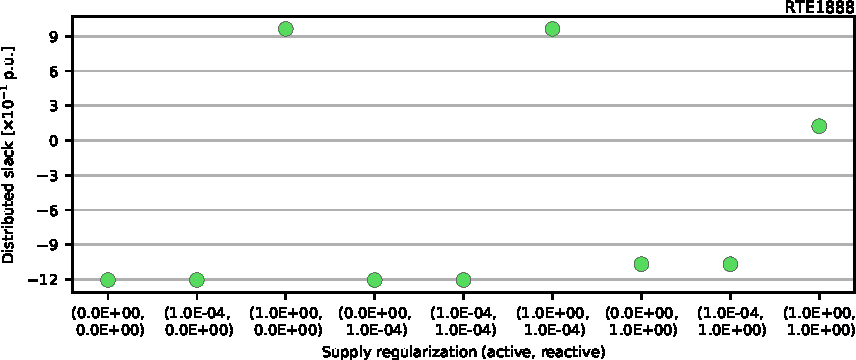
\includegraphics[width=0.95\textwidth]{trick_RTE1888.pdf} \end{figure}
    }
    \onslide*<4>{
    \begin{figure} 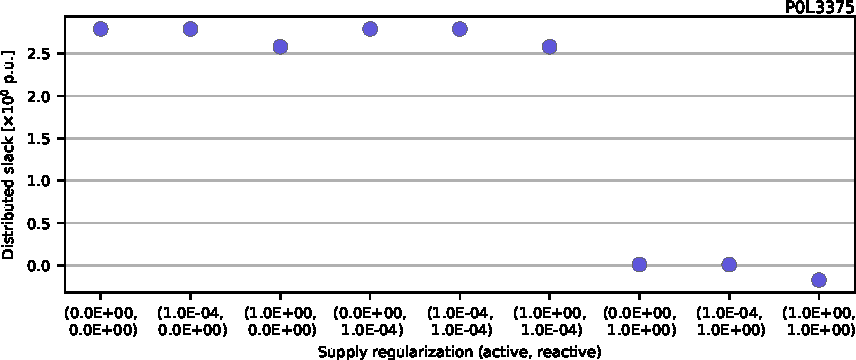
\includegraphics[width=0.95\textwidth]{trick_POL3375.pdf} \end{figure}
    }

    \begin{block}<5->{Quadrimodal effect}
        The APF point \(\APFPoint\) will be {\color{CornellRed}in one of four neighbourhoods}
        in the upcoming-dispatch PFM.
    \end{block}

    \begin{overlayarea}{\textwidth}{\textheight}
    \begin{onlyenv}<6>
    Consider \XED in 1D:
    minimize \(\AbsVal*{x} + \mu\AbsVal*{x-1}\) s.t. \(-3 \leq x \leq 3\), where \(\mu \geq 0\)
    \begin{figure} 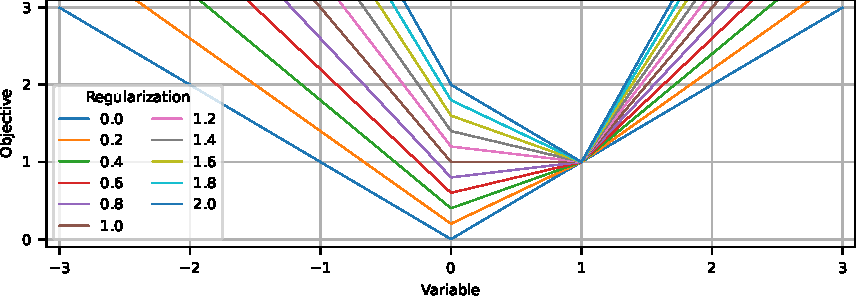
\includegraphics[width=0.95\textwidth]{1d-apf1.pdf} \end{figure}
    \end{onlyenv}

    \begin{onlyenv}<7>
    \begin{corollary}[Big-\(\mu\) trick for finding four APF points]
        Regularizing \XED with
        {\color{CornellRed}
        \(\XEDRegs \in \left\{0,\mu\right\} \times \left\{0,\mu\right\}\),
        for some \(\mu \gg 0\)},
        yields four \(\SupInjs\)'s,
        and, by \APFE, four \(\PFEVars\)'s.
        These {\color{CornellRed}four independent APF instances} can be run in parallel.
    \end{corollary}
    \end{onlyenv}
    \end{overlayarea}
\end{frame}


\section{Applications}
\subsection{Warm-starting an OPF solver}

\begin{frame}[t]{APF for OPF: Providing solvers with warm-start points}{}
    OPF solvers are iterative:
    \textcolor<1>{CornellRed}{\(\OPFVars[k+1] \gets \operatorname{update}\!\OPFVars[k]\)}
    \begin{itemize}
        \item User-specified \textcolor<1>{CornellRed}{starting point \(\OPFVars[0]\)}
        \item \textcolor<1>{CornellRed}{Interior-point methods} are SOTA \cite{Capitanescu+2007},
            especially in large scale \cite{CapitanescuWehenkel2013,Kardos+2020v4,Kardos+2022}
    \end{itemize}

    \onslide*<2->{
    \vspace{1em}
    \textcolor<2>{CornellRed}{Snapshot-starting} a solver
    \begin{itemize}
        \item \(\OPFVars[0] \gets \SnapPoint\)
        \item[\ding{43}] Search \textcolor<2>{CornellRed}{does not start on PFM}
    \end{itemize}
    }

    \onslide*<3->{
    \vspace{1em}
    \textcolor<3>{CornellRed}{Warm-starting} a solver with APF point \(\APFPoint\)
    \begin{itemize}
        \item \(\OPFVar{c}{0} \gets \left(\SupPs + \PFESlack\PFESDist, \SupQs\right)\)
        \item \(\OPFVar{s}{0} \gets \BusMAs\)
        \item[\ding{43}] Search \textcolor<3>{CornellRed}{starts on PFM}
    \end{itemize}
    }
\end{frame}

\begin{frame}[t]{APF for OPF: Providing solvers with warm-start points}{}
    \begin{columns}[T]
    \begin{column}{0.5\textwidth}
    \onslide*<1->{
    Solve instances on \texttt{POL3375} via MIPS 1.4 \cite{MIPSv1.4}
    \begin{itemize}
        \item 408 APF instances

        \item Get snapshot- \& warm-started optima
        \begin{itemize}
            \item \(\Optim[s]{\SupInjs}\), \(\Optim[s]{\BusMs}\), \(\Optim[s]{\BranchAs}\), \(\Optim[s]{g}\)
            \item \(\Optim[w]{\SupInjs}\), \(\Optim[w]{\BusMs}\), \(\Optim[w]{\BranchAs}\), \(\Optim[w]{g}\)
        \end{itemize}

        \item Compare solutions in terms of
        \begin{itemize}
            \item \(\epsilon_{\mathsf{c}} \coloneqq \Norm*{\begin{matrix*}
                \Optim[s]{\SupInjs}-\Optim[w]{\SupInjs}\end{matrix*}}_{\infty}\)
                (in 100-MVA units)
            \item \(\epsilon_{\mathsf{v}} \coloneqq \Norm*{\begin{matrix*}
                \Optim[s]{\BusMs}-\Optim[w]{\BusMs}\end{matrix*}}_{\infty}\)
                (in 400-kV units)
            \item \(\epsilon_{\mathsf{a}} \coloneqq \Norm*{\begin{matrix*}
                \Optim[s]{\BranchAs}-\Optim[w]{\BranchAs}\end{matrix*}}_{\infty}\)
                (in radians)
            \item \(\epsilon_{\mathsf{g}} \coloneqq \Optim[s]{g} - \Optim[w]{g}\)
                (in USD)
        \end{itemize}

        \item[\ding{43}] <7->
            \textcolor<7->{CornellRed}{
            \(\left(\Optim[w]{g},\Optim[w]{\BusMs},\Optim[w]{\BranchAs}\right)
            \approxeq
            \left(\Optim[s]{g},\Optim[s]{\BusMs},\Optim[s]{\BranchAs}\right)\)}
            attained from \textcolor<7->{CornellRed}{
            distinct \(\Optim[w]{\SupInjs}\) and \(\Optim[s]{\SupInjs}\)} 
    \end{itemize}
    }
    \end{column}

    \begin{column}{0.5\textwidth}
    \onslide*<2-7>{
    \hspace*{\fill}{\small At \(\XEDRegs=\left(0,0\right)\)}
    \begin{table}[t!] \vspace{-0.7em} \small
    \begin{tabularx}{\textwidth}{@{} cCC @{}}
    \toprule
    Metric & Minimum & Maximum
    \\ \midrule
    \(\epsilon_{\mathsf{g}}\)
    & \textcolor<3>{BrandeisBlue}{\(-1.7847\times10^{-2}\)}
    & \textcolor<3>{BrandeisBlue}{\(1.90488\times10^{-2}\)}
    \\
    \(\epsilon_{\mathsf{v}}\)
    & \textcolor<4>{LightSalmon}{\(4.79369\times10^{-9}\)}
    & \textcolor<4>{LightSalmon}{\(6.89567\times10^{-5}\)}
    \\
    \(\epsilon_{\mathsf{a}}\)
    & \textcolor<4>{LightSalmon}{\(6.47442\times10^{-10}\)}
    & \textcolor<4>{LightSalmon}{\(5.92979\times10^{-6}\)}
    \\
    \(\epsilon_{\mathsf{c}}\)
    & \textcolor<5-7>{CornellRed}{\(6.05418\times10^{-4}\)}
    & \textcolor<5-7>{CornellRed}{\(8.78352\times10^{-1}\)}
    \\
    \bottomrule
    \end{tabularx}
    \end{table}
    }

    \onslide*<6-7>{
    \hspace*{\fill}{\small At \(\XEDRegs=\left(1,1\right)\)}
    \begin{table}[t!] \vspace{-0.7em} \small
    \begin{tabularx}{\textwidth}{@{} cCC @{}}
    \toprule
    Metric & Minimum & Maximum
    \\ \midrule
    \(\epsilon_{\mathsf{g}}\)
    & \(-1.21094\times10^{-2}\)
    & \(2.14678\times10^{-2}\)
    \\
    \(\epsilon_{\mathsf{v}}\)
    & \(1.82573\times10^{-9}\)
    & \(2.4873\times10^{-5}\)
    \\
    \(\epsilon_{\mathsf{a}}\)
    & \(2.88286\times10^{-10}\)
    & \(3.47572\times10^{-6}\)
    \\
    \(\epsilon_{\mathsf{c}}\)
    & \textcolor<6-7>{CornellRed}{\(1.23703\times10^{-4}\)}
    & \textcolor<6-7>{CornellRed}{\(2.88003\times10^{-1}\)}
    \\
    \bottomrule
    \end{tabularx}
    \end{table}
    }

    \onslide*<8>{
    \hspace*{\fill}{\small At \(\XEDRegs=\left(1,0\right)\)}
    \begin{table}[t!] \vspace{-0.7em} \small
    \begin{tabularx}{\textwidth}{@{} cCC @{}}
    \toprule
    Metric & Minimum & Maximum
    \\ \midrule
    \(\epsilon_{\mathsf{g}}\)
    & \textcolor<8>{BrandeisBlue}{\(-2.44578\times10^{-2}\)}
    & \textcolor<8>{BrandeisBlue}{\(2.24346\times10^{-2}\)}
    \\
    \(\epsilon_{\mathsf{v}}\)
    & \textcolor<8>{LightSalmon}{\(7.57086\times10^{-10}\)}
    & \textcolor<8>{LightSalmon}{\(6.40276\times10^{-5}\)}
    \\
    \(\epsilon_{\mathsf{a}}\)
    & \textcolor<8>{LightSalmon}{\(1.99231\times10^{-10}\)}
    & \textcolor<8>{LightSalmon}{\(4.99960\times10^{-6}\)}
    \\
    \(\epsilon_{\mathsf{c}}\)
    & \textcolor<8>{CornellRed}{\(6.91804\times10^{-4}\)}
    & \textcolor<8>{CornellRed}{\(1.16527\times10^{0}\)}
    \\
    \bottomrule
    \end{tabularx}
    \end{table}
    }
    \end{column}
    \end{columns}
\end{frame}

\begin{frame}[t]{APF for OPF: Providing solvers with warm-start points}{}
    \begin{block}<1->{It's just the nonconvexity of OPF}
        The APF point
        \textcolor<1->{CornellRed}{can be sufficiently far} from the snapshot point
        that, for \textcolor<1->{CornellRed}{the same algorithm},
        these starting points lead to \textcolor<1->{CornellRed}{distinct optima}.
    \end{block}

    \begin{corollary}<2->{}
        In its current form, APF is
        \textcolor<2->{CornellRed}{a crude method for finding multiple OPF solutions}.
    \end{corollary}

    \begin{alertblock}<3->{Open problems}
    \begin{enumerate}
        \item Given a solver, a snapshot point \(S\), and a APF point \(A\),
            how can we tell that starting the solver at \(S\) and at \(A\)
            will or will not give us distinct optima?
        \item How to make APF a more disciplined method of finding multiple OPF solutions?
    \end{enumerate}
    \end{alertblock}
\end{frame}

\subsection{Differentiating through the APF equations}

\begin{frame}[t]{APF for amortized OPF: Differentiating through \APFE}{}
    \onslide*<1->{
    Neural nets to learn solution maps of OPF instances
    with fixed \(\Ybus\) but varying \(\DemDrws\)
    \begin{itemize}
        \item <1-> Design challenge: \textcolor<1>{CornellRed}{differentiably incorporate PFE}

        \item <2-> \textcolor<2>{CornellRed}{OPF-DNN}:
            violation-based Lagrangian relaxation \cite{Chatzos+2020v1}
        \begin{itemize}
            \item \(\DemDrws
                \xrightarrow{\operatorname{Net}_{\boldsymbol{\theta}}\paren{\cdot}}
                \SupInjs,\BusVolts \xrightarrow{\text{computations}}
                \ell = \cdots + \lambda
                \Norm*{\begin{matrix*}\Resids\paren{\SupInjs,\BusVolts}\end{matrix*}}_{1}\)
            \item[\faExclamation] Only encourages PFE compliance
        \end{itemize}

        \item <3-> \textcolor<3>{CornellRed}{DeepOPF}:
            SPF + zeroth-order gradient estimation \cite{DeepOPF-FOACOPFv6}
        \begin{itemize}
            \item \(\DemDrws
                \xrightarrow{\operatorname{Net}_{\boldsymbol{\theta}}\paren{\cdot}}
                \hat{\SupPs},\hat{\BusMs} \xrightarrow{\text{SPF}}
                \SupInjs,\BusVolts \xrightarrow{\text{computations}} \ell\)
            \item[\faExclamation] Inexact gradient could hurt training
        \end{itemize}

        \item <4-> \textcolor<4>{CornellRed}{DC3}:
            SPF + penalty + differentiating through SPF \cite{DC3}
        \begin{itemize}
            \item \(\DemDrws
                \xrightarrow{\operatorname{Net}_{\boldsymbol{\theta}}\paren{\cdot}}
                \hat{\SupPs},\hat{\BusMs} \xrightarrow{\text{SPF}}
                \SupInjs,\BusVolts \xrightarrow{\text{computations}}
                \ell = \cdots + \lambda
                \Norm*{\begin{matrix*}\Resids\paren{\SupInjs,\BusVolts}\end{matrix*}}_{2}^{2}
                \)
            \item[\faExclamation] Differentiating through SPF is (very) complicated
        \end{itemize}
        \end{itemize}
    }
\end{frame}

\begin{frame}[t]{APF for amortized OPF: Differentiating through \APFE}{}
    \begin{exampleblock}<1->{Long-term mission}
        Treating \(\operatorname{Net}_{\boldsymbol{\theta}}\paren{\cdot}\)
        as anticipating \(\SupInjs\),
        we have
        \(\textcolor{CornellRed}{\DemDrws
        \xrightarrow{\operatorname{Net}_{\boldsymbol{\theta}}\paren{\cdot}}
        \SupInjs \xrightarrow{\text{solve \APFE}} \PFEVars \xrightarrow{\text{computations}}
        \ell\paren{\SupInjs,\PFEVars\paren{\SupInjs}}}\)
        for any appropriate loss \(\ell\).
        Backpropagation simply follows
        \textcolor{CornellRed}{
        \(\textcolor{CornellRed}{\odif{\ell} =
        \bigl(\partial_{\SupInjs}\ell + \partial_{\PFEVars}\ell\, \partial_{\SupInjs}\PFEVars\bigr)
        \partial_{\boldsymbol{\theta}}\SupInjs \odif{\boldsymbol{\theta}}}\)}.
    \end{exampleblock}

    \begin{overlayarea}{\textwidth}{\textheight}
    \begin{onlyenv}<2-3>
    \begin{itemize}
        \item <2-3> \(\partial_{\boldsymbol{\theta}}\SupInjs\),
            \(\partial_{\SupInjs}\ell\paren{\cdot}\),
            and \(\partial_{\PFEVars}\ell\paren{\cdot}\)
            are \textcolor<2>{CornellRed}{trivial for modern autodiff engines}

        \item[\ding{43}] <3> Contribution: How to differentiate through \APFE
        \begin{itemize}
            \item <3> Computing the
                \textcolor<3>{CornellRed}{backward APF Jacobian
                \(\APFJac[b]\paren{\cdot} \,\coloneqq \partial_{\SupInjs}\PFEVars\paren{\cdot}\)}
            \item <3> Computing the
                \textcolor<3>{CornellRed}{backward APF gradient
                \(\APFBGrad\paren{\cdot}\)},
                \ie,
                \(\APFBGrad^{\!\mathsf{T}}\paren{\cdot} \,\equiv
                \partial_{\PFEVars}\ell\paren{\cdot}\,\APFJac[b]\paren{\cdot}\)
        \end{itemize}
    \end{itemize}
    \end{onlyenv}

    \begin{block}<4->{Computing the backward APF Jacobian (\S 4.4.1)}
        Applying the implicit function theorem at an APF point \(\APFPoint\),
        the \textcolor{CornellRed}{backward APF Jacobian} is the solution to
        \textcolor{CornellRed}{
        \(\APFJac\paren{\PFEVars}\,\APFJac[b]\paren{\PFEVars} \,= \Diag{\SupCon,\SupCon}\)}.
    \end{block}

    \begin{block}<5->{Computing the backward APF gradient (\S 4.4.2)}
        \textcolor{CornellRed}{Jacobian-vector product} (JVP):
        solve for \(\APFJac[b]\),
        then \(\APFBGrad = \APFJac[b]^{\mathsf{T}} \, \nabla_{\!\PFEVars}\ell\)

        \textcolor{CornellRed}{Vector-Jacobian product} (VJP):
        solve for \(\RealVec{u}\) from
        \(\APFJac^{\mathsf{T}} \RealVec{u} = \nabla_{\!\PFEVars}\ell\),
        then \(\APFBGrad = \Diag{\SupCon^{\mathsf{T}},\SupCon^{\mathsf{T}}} \, \RealVec{u}\)
    \end{block}
    \end{overlayarea}
\end{frame}

\begin{frame}[t]{APF for amortized OPF: Differentiating through \APFE}{}
    \begin{columns}[T]
    \begin{column}{0.4\textwidth}
    Prefer VJP to JVP
    \begin{itemize}
        \item <5-> No need to form \(\APFJac[b]\),
            which is \textcolor<5>{CornellRed}{\(2\NumBuses \times 2\NumSupUnits\) and dense}

        \item <6-> With mild assumptions (\S A.3.2),
        \begin{itemize}
            \item <6-> JVP is \textcolor<6>{CornellRed}{
                \(\bigO\paren{\tfrac{32}{2}\NumSupUnits\NumBuses^{3}}\) flops}
            \item <6-> VJP is \textcolor<6>{CornellRed}{
                \(\bigO\paren{\tfrac{16}{3}\NumBuses^{3}}\) flops}
        \end{itemize}
    \end{itemize}
    \end{column}

    \begin{column}{0.6\textwidth}
    \onslide*<2->{
    {\small
    Gradients are of \(\ell\) in Equation (4.24).
    Wall times are averaged over 100 runs,
    based on Intel Core i7-10750H w/ 16GB RAM.}
    \begin{table}[t!] \vspace{-0.7em} \small
    \begin{tabularx}{\textwidth}{@{} cCCC @{}}
    \toprule
    System
    & \(\Norm*{\begin{matrix*}
        \APFBGrad_{\mathsf{jvp}}-\APFBGrad_{\mathsf{vjp}}\end{matrix*}}_{\infty}\)
    & JVP time [s]
    & VJP time [s]
    \\ \midrule
    \texttt{ACT500}
    & \textcolor<3>{BrandeisBlue}{\(3.9968\times10^{-14}\)}
    & \textcolor<4>{AtomicTangerine}{\(3.3319\times10^{-2}\)}
    & \textcolor<4>{CornellRed}{\(4.4259\times10^{-3}\)}
    \\
    \texttt{RTE1888}
    & \textcolor<3>{BrandeisBlue}{\(7.3630\times10^{-13}\)}
    & \textcolor<4>{AtomicTangerine}{\(5.4983\times10^{-1}\)}
    & \textcolor<4>{CornellRed}{\(1.8315\times10^{-2}\)}
    \\
    \texttt{POL3375}
    & \textcolor<3>{BrandeisBlue}{\(5.5111\times10^{-12}\)}
    & \textcolor<4>{AtomicTangerine}{\(2.4872\)}
    & \textcolor<4>{CornellRed}{\(3.4472\times10^{-2}\)}
    \\
    \bottomrule
    \end{tabularx}
    \end{table}
    }
    \end{column}
    \end{columns}
\end{frame}

\begin{frame}[t]{APF for amortized OPF: Differentiating through \APFE}{}
    \begin{exampleblock}{Long-term mission}
        Treating \(\operatorname{Net}_{\boldsymbol{\theta}}\paren{\cdot}\)
        as anticipating \(\SupInjs\),
        we have
        \(\textcolor{CornellRed}{\DemDrws
        \xrightarrow{\operatorname{Net}_{\boldsymbol{\theta}}\paren{\cdot}}
        \SupInjs \xrightarrow{\text{solve \APFE}} \PFEVars \xrightarrow{\text{computations}}
        \ell\paren{\SupInjs,\PFEVars\paren{\SupInjs}}}\)
        for any appropriate loss \(\ell\).
        Backpropagation simply follows
        \textcolor{CornellRed}{
        \(\textcolor{CornellRed}{\odif{\ell} =
        \bigl(\partial_{\SupInjs}\ell + \partial_{\PFEVars}\ell\, \partial_{\SupInjs}\PFEVars\bigr)
        \partial_{\boldsymbol{\theta}}\SupInjs \odif{\boldsymbol{\theta}}}\)}.
    \end{exampleblock}

    \begin{alertblock}{Open problems and working ideas}
        \begin{enumerate}
            \item How to solve a batch of \APFE instances with GPU acceleration?
            \begin{itemize}
                \item[\faLightbulb] Cast as nonlinear least-squares,
                    then use JAXOpt \cite{Blondel+2022v5}
            \end{itemize}

            \item How to quantify model uncertainty?
            \begin{itemize}
                \item[\faLightbulb] Extend conformal prediction \cite{GenIntroConfPred_v5}
                    into a multivariate regression case
            \end{itemize}
        \end{enumerate}
        \end{alertblock}
\end{frame}


\section{Conclusion}
\begin{frame}[t]{APF in summary}{}
    \begin{itemize}
        \item \textcolor<1>{CornellRed}{Formulation}:
            finding power-flow feasible \(\left(\SupInjs,\BusVolts\right)\)
            for anticipated grid conditions \(\left(\Ybus,\DemDrws\right)\),
            using preceding snapshot values \(\SnapPoint\)
        \begin{itemize}
            \item Anticipate \(\SupInjs\) by solving a convex program
                \textcolor<1>{CornellRed}{\XED[full]} (\XED)
            \item Compute corresponding \(\BusVolts\) by solving
                \textcolor<1>{CornellRed}{\APFE[full]} (\APFE)
        \end{itemize}

        \vspace{0.5em}
        \item \textcolor<2>{CornellRed}{Computation}:
            amply handled by existing and readily available tools
        \begin{itemize}
            \item SeDuMi and SDPT3 for \XED;
                Levenberg-Marquardt and Powell hybrid for \APFE
            \item \textcolor<2>{CornellRed}{Sub-second run times}
                on 3374-bus, 4161-branch, 596-generator portion of Polish grid
            \item \textcolor<2>{CornellRed}{Quadrimodal effect} of \XED
                \(\Longrightarrow\)
                \textcolor<2>{CornellRed}{big-\(\mu\) trick} for easily finding four APF points
        \end{itemize}

        \vspace{0.5em}
        \item \textcolor<3>{CornellRed}{Applications}
        \begin{enumerate}
            \item Warm-starting OPF solvers
                \(\Longrightarrow\)
                \textcolor<3>{CornellRed}{a crude method for finding multiple OPF solutions}

            \item Differentiating through \APFE
                \(\Longrightarrow\)
                \textcolor<3>{CornellRed}{power flow equations as a layer in amortized OPF}
        \end{enumerate}
    \end{itemize}
\end{frame}


\begin{frame} \titlepage \end{frame}

\section{References}
\begin{frame}[t,allowframebreaks]{References}{}
    \printbibliography[heading=none]
\end{frame}

\end{document}
